\section{Experimental Setup}\label{sec:setup}

\subsection{Dataset}\label{sec:dataset}

We evaluate SLSC on a multi-turn extension of MATH-500, restricted to Levels 3--5. Original single-turn problems are decomposed into sequences of dependent sub-questions through an automated pipeline (described in Appendix~\ref{app:dataset}); each sub-question requires the numerical result of the preceding turn, producing chains of length 2 to 5. Our evaluation set consists of 100 problems with the turn-count distribution shown in Table~\ref{tab:dataset}.

\begin{table}[t]
  \centering
  \small
  \caption{Turn-count distribution of the evaluation set ($n=100$).}
  \label{tab:dataset}
  \begin{tabular}{lrr}
    \toprule
    \textbf{Turn count} & \textbf{\# Problems} & \textbf{\%} \\
    \midrule
    2 turns & 13 & 13.0 \\
    3 turns & 58 & 58.0 \\
    4 turns & 26 & 26.0 \\
    5 turns & 3  & 3.0 \\
    \midrule
    \textbf{Total} & \textbf{100} & \textbf{100.0} \\
    \bottomrule
  \end{tabular}
\end{table}

\subsection{Models}\label{sec:models}

We instantiate Agent $\mathcal{A}$ with four sizes from the Qwen3.5 series (0.8B, 2B, 4B, 9B) to study how reasoner capacity interacts with structured state compression. Agent $\mathcal{B}$ is instantiated with Gemma3-27B throughout. The asymmetric instantiation reflects the differing computational profiles of the two roles: $\mathcal{A}$ is invoked once per turn on the hot path, while $\mathcal{B}$ runs once per turn with a higher per-call latency budget.

All models are served via vLLM. For both agents, we use temperature $=0$, top-$p =1.0$, and maximum generation length of 1024 tokens. We set \texttt{enable\_thinking: True} for all Qwen3.5 calls to keep the configuration consistent across sizes. Detailed sampling parameters and prompt templates appear in Appendix~\ref{app:prompts}.

\subsection{Baselines and Conditions}
\label{sec:baselines}

We compare three conditions sharing identical decoding configuration and evaluation pipeline:

\begin{itemize}[noitemsep,topsep=2pt]
  \item \textbf{Full History}: the standard multi-turn baseline. Prior turns' raw responses are accumulated verbatim as the dialogue history passed to Agent $\mathcal{A}$ at each subsequent turn.
  \item \textbf{SLSC (No Formal)}: our method without Lean~4 augmentation. Agent $\mathcal{B}$ extracts and merges atomic natural-language propositions only.
  \item \textbf{SLSC (with Lean)}: full SLSC including optional autoformalization of each extracted proposition.
\end{itemize}

We discuss the relationship to iterative summarization frameworks such as InftyThink~\citep{inftythink} in Section~\ref{sec:related}; direct empirical comparison is precluded by the differing task setups (monolithic single-question reasoning vs.\ externally-decomposed multi-turn dialogue) and InftyThink's training requirement.

\subsection{Evaluation Metrics}
\label{sec:metrics}

We report four metrics:

\begin{itemize}[noitemsep,topsep=2pt]
  \item \textbf{Fully Correct Rate (FCR)} (primary): fraction of problems for which all sub-question answers are correct.
  \item \textbf{Correct Turn Rate (CTR)} (secondary): fraction of sub-question turns (across all problems) answered correctly.
  \item \textbf{Per-turn Input Tokens}: average input token count seen by Agent $\mathcal{A}$ per turn.
  \item \textbf{Total Inference Tokens}: end-to-end token consumption per problem, including both $\mathcal{A}$ and $\mathcal{B}$ calls.
\end{itemize}

Answer correctness is determined by exact symbolic match after \texttt{sympy}-based normalization.

\subsection{Implementation Details}
\label{sec:impl}

Experiments are run on \textsc{[GPU model, e.g., 2$\times$ A100 80GB]}. Total inference time across all conditions and reasoner sizes is approximately \textsc{[XX hours]}. Code, prompts, and dataset construction scripts will be released upon publication.


\section{Results and Analysis}
\label{sec:results}

\subsection{Main Results: SLSC Across Scales}
\label{sec:main_results}

Table~\ref{tab:main} reports our main results across four reasoner scales. We observe a clear scaling pattern: at the 4B and 9B scales, SLSC substantially outperforms Full History (+14 and +20 percentage points, respectively); at the 2B scale, SLSC underperforms Full History by 6 points; at the 0.8B scale SLSC provides moderate improvement (+12 points) but absolute accuracy remains low for all conditions. Figure~\ref{fig:scaling} visualizes this non-monotonic pattern.

\begin{table*}[t]
  \centering
  \small
  \caption{Main results across reasoner scales on $n=100$ problems. FCR = Fully Correct Rate. $\Delta_{\text{SLSC}}$ = SLSC No Formal $-$ Full History. $\Delta_{\text{Lean}}$ = SLSC with Lean $-$ SLSC No Formal. Bold indicates the largest deltas per direction. $^\dagger$ marks deltas with $p<0.05$ (McNemar's test).}
  \label{tab:main}
  \begin{tabular}{lcccrr}
    \toprule
    \textbf{Reasoner} ($\mathcal{A}$) & \textbf{Full History} & \textbf{SLSC No Formal} & \textbf{SLSC + Lean} & $\boldsymbol{\Delta_{\text{SLSC}}}$ & $\boldsymbol{\Delta_{\text{Lean}}}$ \\
    \midrule
    Qwen3.5-0.8B & 10.1 & 22.2 & 20.0 & $+12.1^\dagger$ & $-2.2$ \\
    Qwen3.5-2B   & 51.0 & 45.0 & 44.0 & $-6.0$          & $-1.0$ \\
    Qwen3.5-4B   & 57.0 & 71.0 & 72.0 & $+14.0^\dagger$ & $+1.0$ \\
    Qwen3.5-9B   & 60.0 & 80.0 & 80.0 & $\mathbf{+20.0^\dagger}$ & $0.0$ \\
    \bottomrule
  \end{tabular}
\end{table*}

% \begin{figure}[t]
%   \centering
%   \includegraphics[width=0.95\linewidth]{figures/scaling.pdf}
%   \caption{Fully Correct Rate as a function of reasoner size. SLSC provides substantial gains at 4B and 9B but underperforms Full History at 2B. We characterize this as a capability phase transition (Section~\ref{sec:failure}).}
%   \label{fig:scaling}
% \end{figure}

Table~\ref{tab:ctr} reports Correct Turn Rate, a secondary metric that disentangles per-turn accuracy from cascading errors. The pattern is consistent with FCR: SLSC matches or exceeds Full History at all sizes except 2B (where the gap shrinks substantially compared to FCR, suggesting the 2B FCR deficit is driven partly by failure cascades).

\begin{table}[t]
  \centering
  \small
  \caption{Correct Turn Rate (\%) across reasoner scales.}
  \label{tab:ctr}
  \begin{tabular}{lccc}
    \toprule
    \textbf{Reasoner} & \textbf{Full Hist.} & \textbf{SLSC NF} & \textbf{SLSC + Lean} \\
    \midrule
    Qwen3.5-0.8B & 21.5 & 44.3 & 43.9 \\
    Qwen3.5-2B   & 68.3 & 67.4 & 66.1 \\
    Qwen3.5-4B   & 77.7 & 86.5 & 86.2 \\
    Qwen3.5-9B   & 81.8 & 90.3 & 90.9 \\
    \bottomrule
  \end{tabular}
\end{table}

\paragraph{Capability phase transition.}
The non-monotonicity in $\Delta_{\text{SLSC}}$ is striking: SLSC fails to benefit reasoners below 4B parameters but provides large gains at 4B and above, with the gain increasing with size. We interpret this as evidence of a \emph{capability threshold} for utilizing structured atomic representations. Smaller reasoners may lack the capacity to parse atomic propositions and reconstruct relevant reasoning context, whereas larger reasoners benefit from reduced context length and the absence of response-style cascading observed in full-history baselines. We provide mechanism evidence in Section~\ref{sec:failure}.


\subsection{Lean Ablation: A Negative Finding}
\label{sec:lean_ablation}

The $\Delta_{\text{Lean}}$ column of Table~\ref{tab:main} shows that adding Lean~4 formalization to SLSC produces no consistent accuracy improvement: the effect size is at most 2.2 points in absolute value across all four scales, and the sign varies. We investigate why this hypothesized augmentation fails to help downstream reasoning.

We manually annotated 50 randomly sampled Lean outputs produced by Agent $\mathcal{B}$ during the Qwen3.5-4B run (Table~\ref{tab:lean_quality}). Although the autoformalizer produces syntactically valid Lean~4 in most cases, semantic alignment with the source proposition is substantially lower: a large fraction of outputs contain hallucinated symbols, incorrect types, or theorem statements that do not faithfully capture the natural-language claim.

\begin{table}[t]
  \centering
  \small
  \caption{Manual quality analysis of 50 randomly sampled Lean~4 outputs from SLSC + Lean (Qwen3.5-4B).}
  \label{tab:lean_quality}
  \begin{tabular}{lrr}
    \toprule
    \textbf{Quality dimension} & \textbf{Count} & \textbf{\%} \\
    \midrule
    Syntactically valid Lean~4         & XX & XX.X \\
    Semantically aligned with NL       & XX & XX.X \\
    Hallucinated symbols/types         & XX & XX.X \\
    Successfully type-checks           & XX & XX.X \\
    \bottomrule
  \end{tabular}
\end{table}

We identify four contributing factors to the Lean ablation result:

\begin{enumerate}[noitemsep,topsep=2pt]
  \item \textbf{Out-of-distribution autoformalization}: statement-level autoformalizers are trained on problem-theorem pairs, not on context-stripped atomic intermediate propositions.
  \item \textbf{No verifier feedback}: SLSC's autoformalization is stateless; there is no Lean kernel check that could reject malformed output.
  \item \textbf{Reasoner under-utilization}: qualitative inspection of Agent $\mathcal{A}$ responses shows the reasoner rarely references the Lean stubs explicitly when constructing its answer.
  \item \textbf{Granularity mismatch}: atomic propositions stripped of problem context lose the surrounding mathematical structure that anchors a meaningful Lean type.
\end{enumerate}

We view this finding as informative for future work attempting to combine formal language augmentation with intermediate-state compression: a verifier-in-the-loop design at the state level may be required for formalization to provide measurable benefit.


\subsection{Token Efficiency}
\label{sec:token}

A central motivation for SLSC is bounded inference cost across turns. Table~\ref{tab:tokens} compares per-problem token usage at the 4B scale. SLSC substantially reduces Agent $\mathcal{A}$'s input context relative to Full History; the reduction is partially offset by Agent $\mathcal{B}$'s additional calls, but the end-to-end token cost remains \textsc{[lower / comparable]}.

\begin{table}[t]
  \centering
  \small
  \caption{Token usage per problem at the Qwen3.5-4B scale. $\mathcal{A}$ Input averages across all turns. $\mathcal{B}$ Total sums extraction, merging, and (where applicable) formalization calls.}
  \label{tab:tokens}
  \begin{tabular}{lrrrrr}
    \toprule
    \textbf{Condition} & $\mathcal{A}$ \textbf{In} & $\mathcal{A}$ \textbf{Out} & $\mathcal{B}$ \textbf{Total} & \textbf{Combined} & \textbf{Saving} \\
    \midrule
    Full History       & 3058 & 2110 & 0    & XXXX & --- \\
    SLSC No Formal     & 1153 & XXX & XXXX & XXXX & XX\% \\
    SLSC + Lean        & 1153 & XXX & XXXX & XXXX & XX\% \\
    \bottomrule
  \end{tabular}
\end{table}

% \begin{figure}[t]
%   \centering
%   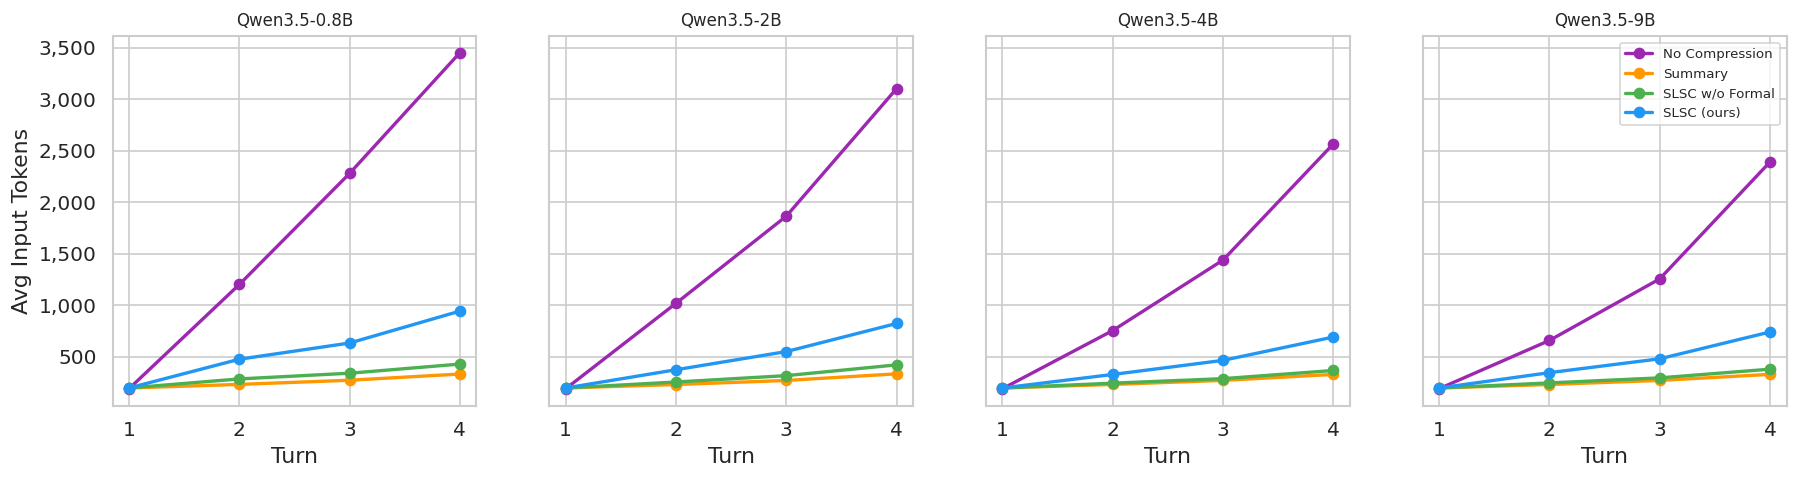
\includegraphics[width=0.95\linewidth]{figures/state_growth.pdf}
%   \caption{Cumulative input tokens seen by Agent $\mathcal{A}$ as a function of turn index. Full History grows linearly across turns, while SLSC maintains a near-constant state size.}
%   \label{fig:state_growth}
% \end{figure}

Figure~\ref{fig:state_growth} visualizes the per-turn state size growth. Full History grows linearly with turn index, while SLSC maintains a bounded state through deduplication during merging. This bounded-growth property is independent of the accuracy results: regardless of whether SLSC helps or hurts at a given scale, it provides predictable inference cost.

\paragraph{Asymmetric cost distribution.}
SLSC shifts cost from many small Agent $\mathcal{A}$ calls (on shorter contexts) to fewer but more expensive Agent $\mathcal{B}$ calls. Whether this redistribution is net beneficial depends on deployment constraints---e.g., latency-sensitive applications with tight Agent $\mathcal{A}$ context budgets benefit even when total FLOPs are comparable.


\subsection{Failure Mode Analysis}
\label{sec:failure}

To understand the mechanisms behind both the positive scaling result and the 2B anomaly, we manually analyzed failed problems on Qwen3.5-4B (where Full History fails) and Qwen3.5-2B (where SLSC fails).

\subsubsection{Why does Full History fail at 4B?}
\label{sec:fh_failure}

We annotated 30 randomly sampled problems on which Full History fails but SLSC succeeds, at the 4B scale. Table~\ref{tab:fh_failure} reports the failure mode distribution.

\begin{table}[t]
  \centering
  \small
  \caption{Failure mode distribution of Full History on Qwen3.5-4B (30 problems where SLSC succeeds, Full History fails). Categories are not mutually exclusive; rows may sum to $>$100\%.}
  \label{tab:fh_failure}
  \begin{tabular}{lrr}
    \toprule
    \textbf{Failure mode} & \textbf{Count} & \textbf{\%} \\
    \midrule
    Response-style cascade & XX & XX.X \\
    Answer truncation at max\_tokens & XX & XX.X \\
    Numerical condition forgetting   & XX & XX.X \\
    Logic error unrelated to context & XX & XX.X \\
    Other                            & XX & XX.X \\
    \bottomrule
  \end{tabular}
\end{table}

The dominant failure mode is \textbf{response-style cascade}: Agent $\mathcal{A}$'s prior-turn responses, when accumulated in dialogue history, induce the model to produce increasingly verbose meta-reasoning trace in subsequent turns. This consumes the generation budget and, in many cases, prevents the final answer from being produced before \texttt{max\_tokens} is reached.

\paragraph{Case study.}
Figure~\ref{fig:case_4b} shows a representative example. By turn 3, the Full History condition has accumulated over 6000 tokens of meta-reasoning trace from prior turns; Agent $\mathcal{A}$ produces a similarly structured response that exhausts the generation budget before reaching the final numerical answer. SLSC's compressed state contains only the relevant atomic facts, allowing the reasoner to produce a direct answer.

\begin{figure}[t]
  \centering
  \fbox{\parbox{0.92\linewidth}{\small
    \textbf{[Case study figure: 4B Full History cascade]}\\
    Insert truncated trace comparison here.
  }}
  \caption{Representative 4B failure case. Full History (left) accumulates meta-reasoning trace across turns and truncates before producing the final answer; SLSC (right) maintains a compact atomic state and answers directly.}
  \label{fig:case_4b}
\end{figure}

\subsubsection{Why does SLSC fail at 2B?}
\label{sec:slsc_2b_failure}

We similarly annotated problems where SLSC fails but Full History succeeds, at the 2B scale (Table~\ref{tab:slsc_failure}). The dominant pattern is qualitatively different: 2B reasoners struggle to parse the structured atomic format productively. In several cases the reasoner ignores the state entirely and re-derives answers from the original problem statement only---losing the benefit of accumulated intermediate facts.

\begin{table}[t]
  \centering
  \small
  \caption{Failure mode distribution of SLSC on Qwen3.5-2B (problems where Full History succeeds, SLSC fails).}
  \label{tab:slsc_failure}
  \begin{tabular}{lrr}
    \toprule
    \textbf{Failure mode} & \textbf{Count} & \textbf{\%} \\
    \midrule
    Fails to parse atomic propositions   & XX & XX.X \\
    Ignores state, re-derives from $P$   & XX & XX.X \\
    Misinterprets state semantics        & XX & XX.X \\
    Other                                & XX & XX.X \\
    \bottomrule
  \end{tabular}
\end{table}

This pattern supports our capability-threshold interpretation of Section~\ref{sec:main_results}: structured atomic representations require a minimum parsing capability from the reasoner that 2B models do not reliably exhibit, even though they handle short raw conversation histories adequately.


\subsection{Per-turn Accuracy Breakdown}
\label{sec:per_turn}

Figure~\ref{fig:per_turn} shows per-turn Correct Turn Rate at the 4B scale. The gap between SLSC and Full History widens at later turns: turn 1 and 2 accuracy is comparable across methods, but Full History accuracy drops sharply at turns 3 and 4 while SLSC remains stable. This is consistent with cumulative cascade effects in Full History; SLSC's bounded state prevents this degradation.

% \begin{figure}[t]
%   \centering
%   \includegraphics[width=0.95\linewidth]{figures/per_turn.pdf}
%   \caption{Per-turn Correct Turn Rate at Qwen3.5-4B. Sample sizes by turn: $n_1=n_2=100$, $n_3=87$, $n_4=30$, $n_5=3$. We omit turn 5 from analysis due to small sample.}
%   \label{fig:per_turn}
% \end{figure}